\documentclass[fancyheadings,11pt]{book}

\usepackage[dvips,pdftex,final]{graphicx}
\usepackage[english]{babel}

\usepackage{amsfonts}
\usepackage{epsfig}
\usepackage{epstopdf}
\usepackage{enumitem}
\usepackage{amssymb,amsmath}
\usepackage{multirow}
\usepackage{natbib}
\bibliographystyle{plainnat}
%\usepackage{hyperref}

\usepackage{enumitem}
\setlist{nosep}


\hyphenation{}
\newtheorem{example}{Example}
\newtheorem{theorem}{Theorem}

\newcommand{\cl}{{\scriptstyle{\it class}}}
\newcommand{\var}{{\mathrm{var}}}
\newcommand{\code}[1]{{\texttt{#1}}}


\DeclareGraphicsExtensions{.eps}


\evensidemargin=1.5cm
\oddsidemargin=1.5cm

\begin{document}

\begin{center}
\thispagestyle{empty}
 \ \ \

\bigskip
\bigskip

{\huge
\textsc{A VTL PROOF OF CONCEPT}
}

\vspace{0.5 cm}
\textsc{\today}

\vspace{1.8 cm}
\textsc{\Large Mark van der Loo, Michael Schaefer\\and Olav ten Bosch}


\vspace{2 cm}
\textsc{\Large DRAFT}

\end{center}

\newpage
\thispagestyle{empty}

\frontmatter
\tableofcontents

%\chapter*{Preface}
%\label{preface}
%\input{preface.tex}

\mainmatter

\chapter{Introduction}
\label{introduction}
\textsc{Mark van der Loo and Michael Schaefer}
\vspace{0.6 cm}

The evaluation of existing languages for specifying data validation rules is
one of the main objectives of the ESSnet on Validation project \citep{ESS:2015}. Specifically, two types of tasks are defined in work package 4,
namely the conduction of a formal study (task 15), described in [study] and the
implementation of a prototype, described in \textsc{this document}. Originally,
two candidate languages were considered for evaluation: VALS, which had already
been under development for some years under the auspices of Eurostat, and VTL,
a more recent development from the SDMX community, of which Eurostat is a
member. Given to circumstances not foreseeable at the outset of the project, the
development of VALS was ceased. This is described in more detail in the
introduction to [study].

The objective of the prototype described in this document was to assess the
practical usability of VTL when used for specifying and exchanging validation
rules in the ESS. Given the current lack of editors and runtimes for VTL, it
was decided to spin the prototype more into the direction of a practical
approach to integrating VTL into existing data validation systems. Fortunately,
two of the project partners, the Dutch CBS and the German FSO, have developed
productive data validation systems -  \textit{Validate} and
\textit{eSTATISTIK}, respectively - that both feature full-fledged data
validation specification languages, but differ fundamentally in their technical
layouts and integrations with end-users and production systems. Including both
systems into the prototype suggested itself as it promised to increase the
relevance of the findings considering the diversity of environments in which
data validation is performed in the ESS.


\chapter{Layout of the PoC}
\label{layoutpoc}
\noindent
\title{Layout of the PoC}


sasasasa

\chapter{Data and Rules}
\label{datarules}
\noindent
\title{Data and Rules}
\label{datarules}

sasasasasa

\chapter{Implementations}
\label{implementations}
\noindent
\title{Implementations}

\vspace{0.6 cm}

\noindent
This chapter presents the various implementations of the data validaion rules described in chapter \ref{implementations}.

\section{VTL}

VTL

\section{Validate}

The \code{validate} package \citep{loo:2015} is build on top of the popular and
R language for statistical computing \citep{rcore:2015}. It is
implemented as an `R package' -- a strictly standardized way of distributing R
software, and publicly available through the Comprehensive R Archive Network
(CRAN). 

\subsubsection{The R language and environment}
The R language is an open source project, supported by the R foundation seated
in Vienna, Austria\footnote{\code{https://www.r-project.org/foundation/}}.
Over the last decade R received a surge in popularity both from research and
data science and business analytics communities. As a result R currently
integrates with every popular software system for data storage and processing,
including Microsoft SQL server, Oracle databases, Tibco Spotfire, Spark, and
Hadoop to name but a few.  Interaction with other programming environments such
as \code{C} and \code{C++}, \code{Java}, \code{.Net}, and \code{javascript} are
readily and freely available as well. The recently established R
consortium\footnote{\code{https://www.r-consortium.org/}} is an industry
initiative aimed to streamline and fund further developments in R.


The validate package is intended to be a small and powerful package that can be
used standalone by an analyst using R, or integrated easily into bigger
projects using one of the facilities mentioned above. As such, it is build with
strong adherence to the famous Unix
philosophy\footnote{\code{https://en.wikipedia.org/wiki/Unix\_philosophy}}: do
one thing, and do it really well.


\subsubsection{Approach for validate}
The philosophy behind the validate package is to reuse existing solutions as
much as possible. Most importantly, this means that rather than defining a
language from scratch, the validate package utilizes a subset of existing R
syntax for defining data validation rules. As an example, consider the following rule from the ESSnet survey \citep{walsdorfer:2015}.
\begin{quote}
Check whether the relative occurrence of the category high in a column
containing values low, high, medium does not exceed 10%.
\end{quote}
We assume a simple test dataset, with at least a column called \code{level}.
\begin{center}
\begin{tabular}{|c|}
\hline
\textbf{level}\\
\hline
medium\\
\hline
low\\
\hline
medium\\
\hline
medium\\
\hline
high\\
\hline
$\vdots$\\
\hline
\end{tabular}
\end{center}
In validate, the above rule translates to the following syntax.
\begin{verbatim}
  counts :=  table(level)
  counts["high"] < 0.1 * sum(counts)
\end{verbatim}
Here, \code{table} is a cross tabulation function that tabulates occurrences
of values in the \code{level} column. Since this function is a standard R
feature, tabulation or counting is not part of validate's syntax. Indeed the
validate package only makes sure that the statements issued by a user are in
fact validating statements as defined in the Handbook on validation developed
for this project \citep{zio:2015}. In particular, this means that every
(statistical) transformation available to R can be part of a validating
statements.  With thousands of functions in base R, combined with the more than
7600 user-contributed packages available on CRAN, this results in a truly rich
set of validation functionality with a minimal cost of development and
maintenance to the authors.

Finally, we note that the approach of reusing R syntax for a specific purpose
is not new. Indeed several authors have created popular packages using the same
technology. Examples include an implementation of the famous grammar of
graphics \citep{wilkinson:2006} by \citet{wickham:2014}, the  `formula
interface' for statistical model specification and a grammar for data
manipulation by \cite{wickham:2014}. In fact, reusing existing languages, in
particular functional languages like R, is a well-established technique in
computer science.  Some key references for developing such embedded domain
specific languages (DSL) are \cite{fowler:2011} and \cite{gibbons:2015}.


\subsubsection{Features and usage}
Given that statistical functionality comes for free with R, the validate
package focuses only on features directly related to execution and maintenance
of validation rules and  analyses and presentation of validation results.
A few of the features are highlighted below.

\begin{description}
\item[Rule definition.] Rules can be defined on the R commandline for interactive
use or in text files that can be stored and manipulated as source code. Rule sets
may also be stored in a data base, since R by default supports connectivity to 
(nearly) any database that is (commercially) available.

\item[Rule metadata.] If so desired, rules can be provided with metadata such as
a time stamp, short and long descriptions, and the origin of the rule.  By
default, validate uses the widely supported YAML format for metadata
\citep{ben:2009}, mainly beacause of its human-readability. Since YAML can be
translated to formats like XML or JSON at the push of a button, communication
of rules between different softwares or machines is very easy.

\item[Rule organisation.] Dependencies between text files defining rules are
supported to allow for easy reuse of rules across different datasets.  A type
of \code{include} statement allows for hierarchical dependencies between rule
sets.

\item[Rule execution.] Validation rules can be confronted with any data that can
be read into R, which encompasses every common data format currently in use.
Of particular interest is \code{SDMX}, which is supported for R through a
package of \cite{bondel:2015}.

\item[Rule analyses.] Automatic detection of rule types, variable occurrence and
the rule dependency graph are currently built in. Add-on packages are currently
prototyped that will allow for detection of redundancies or contradictory rule
sets.

\item[Extensibility.] This is borrowed from R's extensibility. Users may define
functions which can be used in validating statements. The package needs no special
provisions for that.

\item[Integration.] Integration and communication with other is borrowed from
the strong features that R already has in this area. Because of its openness,
many interfaces with existing software and platforms, including commercial
ones, have been developed.

\item[Analyses of results.] The package has basic functionality to aggregate and
visualize results of validation  procedures. For example, one can sort records
according to the number of rule violations (record prioritization) or rules
according to which have been violated most often. Such summaries, and visualisations
thereof are important tools for monitoring data quality and the efficacy of 
data cleaning process steps \citep{pannekoek:2014}.
\end{description}

The \code{validate} package is the successor of an earlier package of the same
authors named \code{editrules}. The latter package has been used in production
for several years at Statistics Netherlands and is being evaluated by several
other national statistical institutes. At the moment, validate is being
introduced as editrules' replacement. The validate package is backwards
compatible with editrules in that it can read the same input files. However,
validate extends the earlier package by allowing for a much wider range of
validation rules (editrules was restricted to certain types of in-record
validation rules that are suitable for an error-localization algorithm).




\section{eSTATISTIK}

\subsubsection{The wider context}
The term \textit{eSTATISTIK} stands for a wider modernisation approach in German official statistics that has been ongoing for more than a decade and that aims at organising the transition from paper based to electronic production workflows and at the same time maximising its benefits in terms of efficiency, cost-effectiveness, flexibility, speed and quality. It involves all 15 German statistical institutes and therefore faces many issues that appear in a similar fashion at the European and international level. From a strategic perspective, standardisation in general and the movement from stove-pipe to cross-domain processes are important elements. This has led to the creation of generic applications and XML document types covering most steps of the production process. Specifically, the data collection process can be fully implemented using only generic metadata-driven applications, including data validation components for front-end and back-end systems.

Another important strategic element is the consolidation and optimisation of the collaboration of the official statistical institutes and their partners. Its implementation requires adequate infrastructures for sharing and exchanging data and metadata throughout development and production life cycles, application hosting and sharing and the avoidance of duplicate work.

In the development and deployment phase, metadata are generated by tools used by domain experts for describing data sets, variables, validation rules and more. Metadata are deployed at specific metadata servers where they are accessible to internal production systems and partly to external users. This metadata infrastructure supports identifiers at the survey level, versioning and partitioning along observation areas (for accommodating resources specific to a single statistical institute). 

\subsubsection{Tools and infrastructure}


For data validation, a number of generic design and production tools exist. Figure~\ref{estattools} shows how those tools interact through the metadata infrastructure and the exchange of XML documents:

\begin{figure}[!ht]
\begin{center}
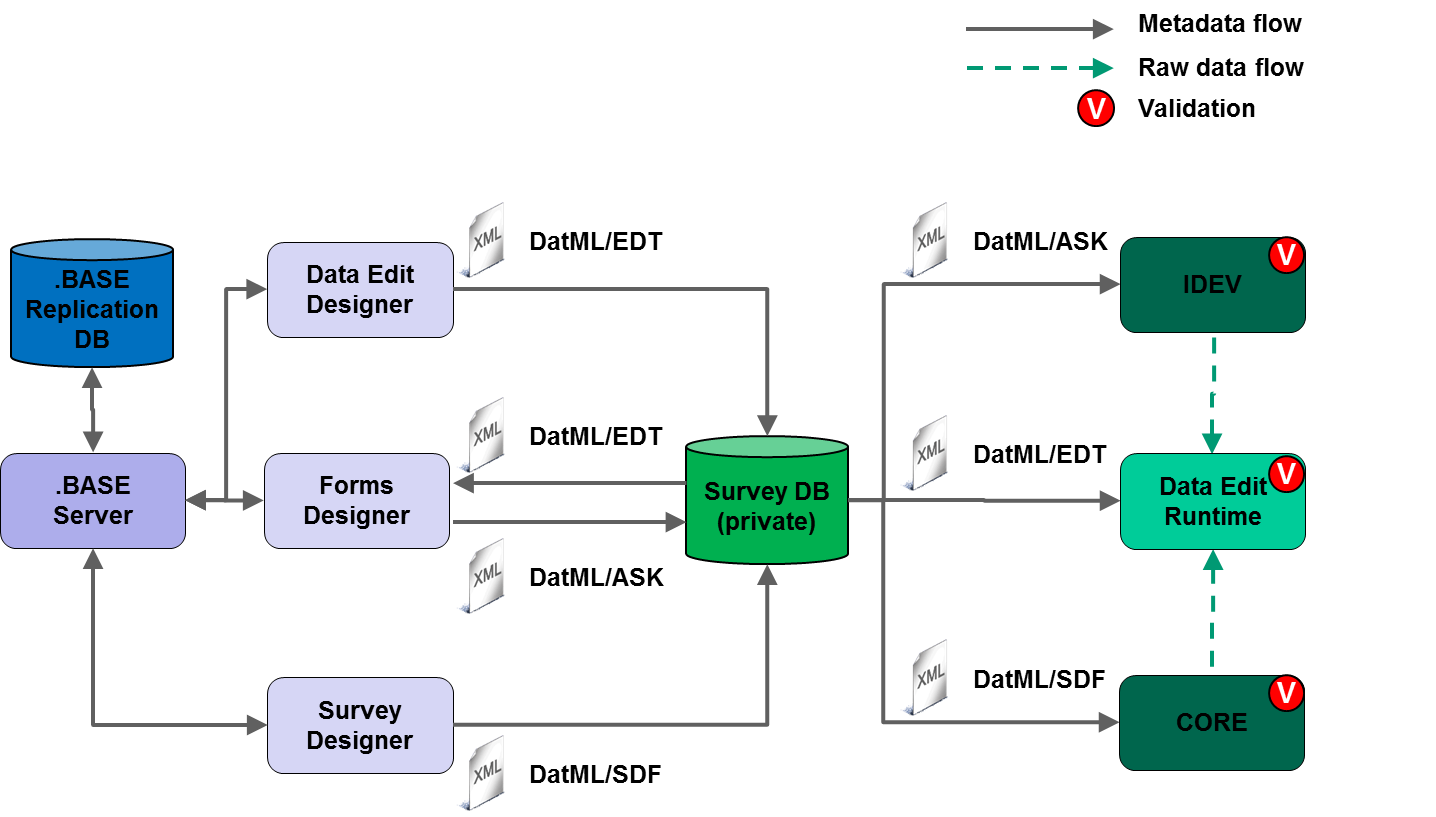
\includegraphics[scale=0.5]{fig/estattools.png} 
\end{center}
\caption{eSTATISTIK tools and their interaction}
\label{estattools}
\end{figure}

\begin{itemize}

\item
Domain experts use \textit{Data Edit Designer} for specifying data models for validation and editing (consisting of variables and variables groups, called \textit{topics}) and validation rules which are mainly used in web forms and back-end systems. Those specifications are exported in \textit{DatML/EDT} format. Validation rules can also be exported as Java classes.

\item
The \textit{Forms Designer} is used for designing web (and paper) forms. It resues data model and rule specifications made with the Data Edit Designer. Forms pecifications are exported in \textit{DatML/ASK} format.

\item
The \textit{Survey Designer} is used for specifying survey data models and front-end validation rules for the B2B data collection system \textit{CORE}.

\item
The \textit{Date Edit Runtime} is a generic platform for perfoming data validation. It is configured through DatML/EDT documents which are deployed along with data to be validated.

\end{itemize}

The design tools are part of the \textit{.BASE} tool suite. They are run as clients of a local .BASE server that provides central storage for metadata objects. A replication database is used for distributing metadata objects among statistical institutes. .BASE servers and the replication database provide the infrastructure for distributed development.

The \textit{Survey Database} serves metadata objects in XML format to production systems. A separate external instance of this database can be accessed by external users, specifically IT service and product providers and respondents.

Figure~\ref{estatinfra} shows the overall infrastructure for the data collection design and production processes:

\begin{figure}[!ht]
\begin{center}
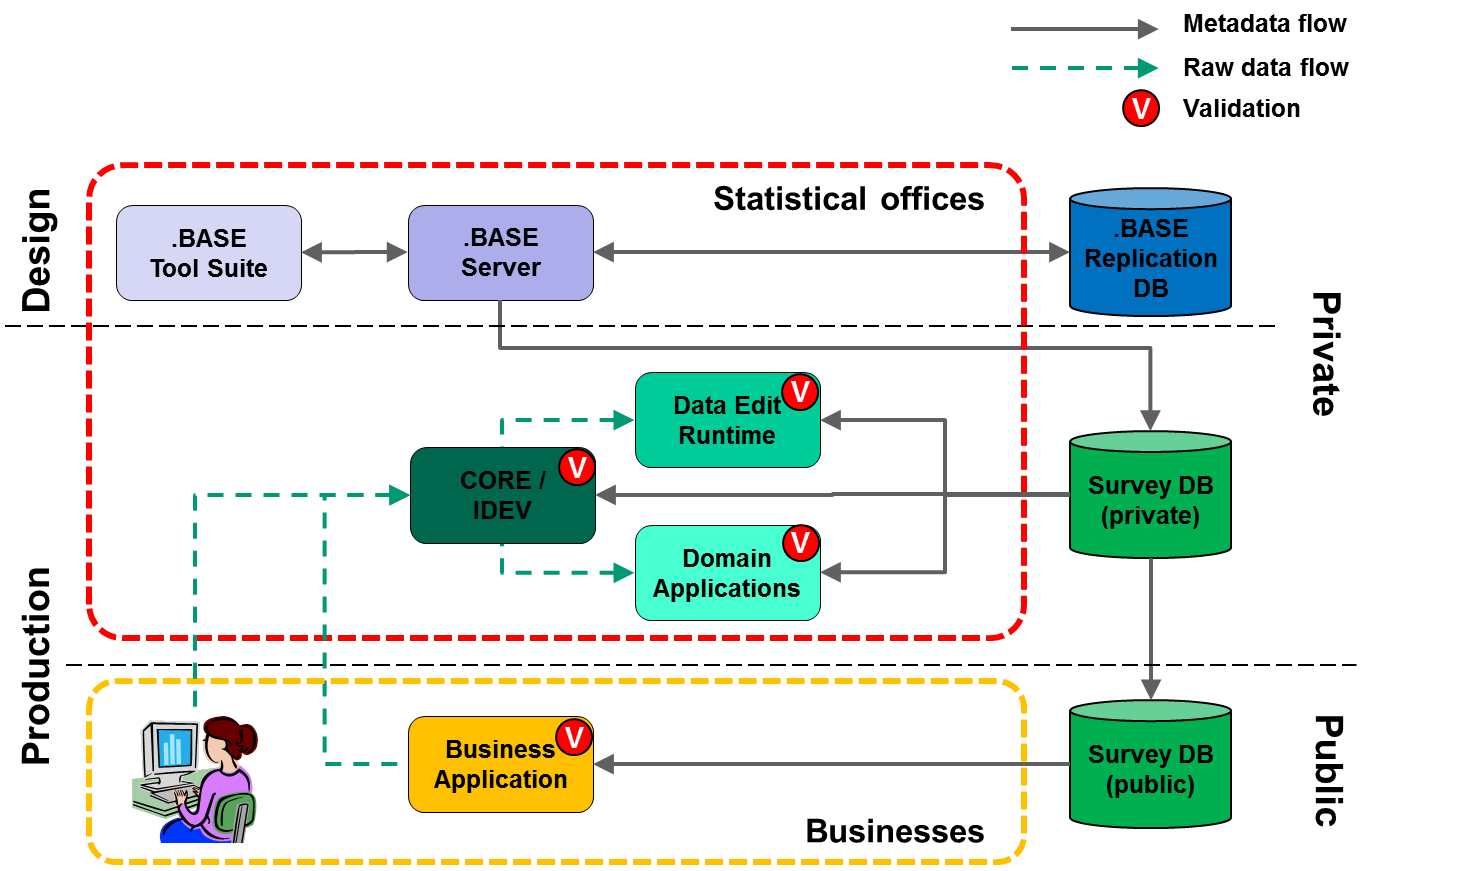
\includegraphics[scale=0.5]{fig/estatinfra.png} 
\end{center}
\caption{eSTATISTIK infrastructure for data collection design and production}
\label{estatinfra}
\end{figure}

\subsubsection{Specification language}

The eSTATISTIK specification language provides instructions for validating and editing data. There exist five fundamental programmatical objects falling into the categories of control, assertion and manipulation, and reuse, as shown in figure~\ref{estatspecl}:

\begin{figure}[!ht]
\begin{center}
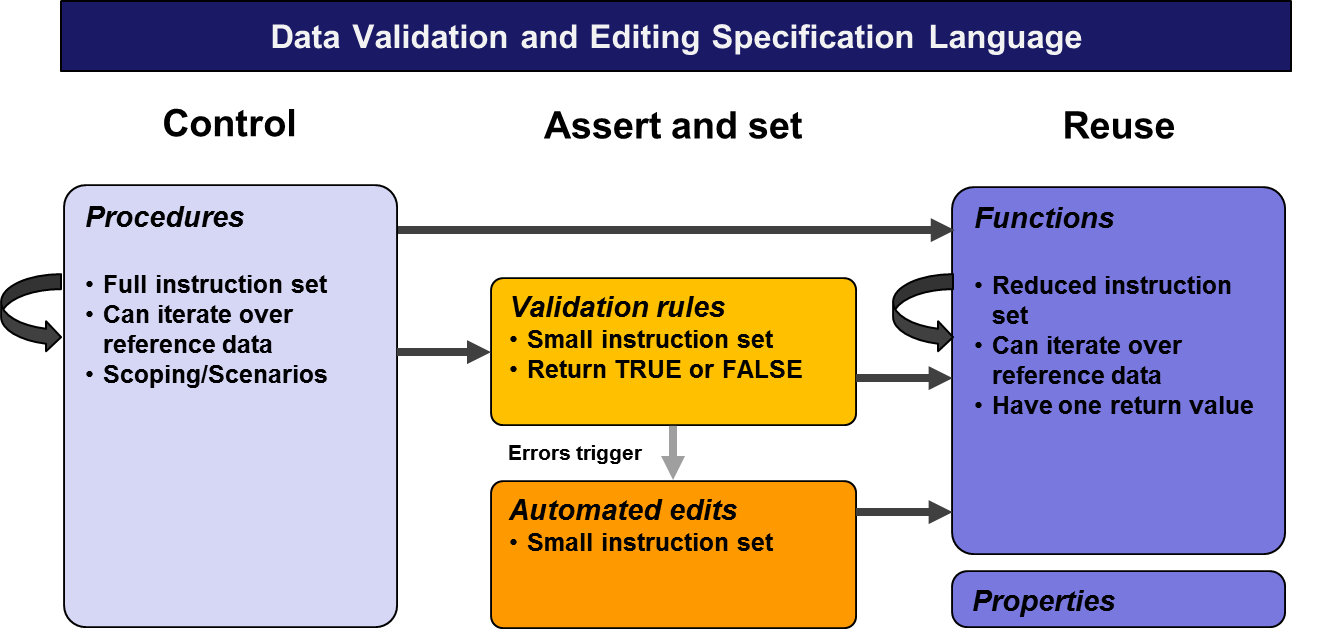
\includegraphics[scale=0.5]{fig/estatspecl.png} 
\end{center}
\caption{eSTATISTIK data validation and editing specification language}
\label{estatspecl}
\end{figure}

Awarenesss of those contexts is very important since they correspond to named programmatic objects that are edited and managed separately in the Data Edit Designer and Data Edit Runtime. They have different and overlapping instruction subsets, but some coding and runtime interdependencies apply.

\begin{description}

\item[Procedures] serve to control the execution path of validation rules and automated edits, or in other words, to create and execute validation flows. Procedures can use the full instruction set of the specification language. Procedures can invoke other procedures conditionally as well as unconditionally, so that validation flows can be scoped and designed as building blocks, providing a means for modularisation and composition of data validation flows.

\item[Checks](a.k.a. validation rules) contain instructions for validating one or more columns/fields of the (hierarchical set of) record(s) currently in scope. Checks can only be invoked from procedures and have a very limited instruction set. They return TRUE if, and only if they encounter an error, otherwise FALSE. Only checks are evaluated for compiling validation statistics or metrics.

\item[Edits] are only invoked implicitly by checks that encounter an error (hard check). There is no instruction for invoking edits explicitly. An edit rule is therefore always bound to exactly one check and also has a very limited instruction set.

\item[Functions] provide a way for creating reusable units of code. Functions dispose of the full instructions set expect that checks cannot be invoked from functions. Functions can be invoked everywhere and recursively.

\end{description}

\paragraph{}
In order for a validation scenario to be executable, at least one rule and one procedure invoking the rule must exist.

\subsubsection{Performing data validation}

In the generic execution environment Data Edit Runtime, programmatic objects such as validation rules, reference data and other resources are bound to a survey node. Different versions of one resource can exist. A survey is associated with one or more reference periods. Reference periods serve to associate the data to be validated with (a version of) the resources used to perform the validation. For a given reference period, exactly one data set under validation can exist.

During execution of a validation flow, only the current record or the current set of hierarchical records (such as household and associated person records) of the data set under validation is visible and can be read and write accessed. Iterating over a complete data set is only possible in procedures and functions and if the data set is defined as reference data.

The Data Edit Runtime is the preferred tool for many small and medium size surveys as it provides full data validation functionality without any need for programming. However, its performance still has to be improved to make it suitable for large data volumes. Bigger surveys typically perform data validation inside the domain application but integrate validation rules defined in the Data Edit Designer through its Java export mechanism.

\subsubsection{Particularities of the PoC}

Files that serve as procedures have control in their file name, while all other .txt files represent simple validation rules.


The data used in the PoC provide some cases in which validation cannot be performed due to missing data. Those cases are recognisable by the value \code{undecided} in the column \code{expected} or in the data set name (where the full data set is validated), respectively. The idea behind this is to find out how systems differ in handling missing values. In eSTATISTIK, after executing a validation rule, the associated data are always considered validated, because validation rules only return TRUE or FALSE. Any precondition that may lead to a validation rule not being executed must be checked outside the rule, that is, in a procedure. For a detailed explanation, please see the eSTATISTIK implemenation of Rule 01
in \ref{appendix}.


\chapter{Results}
\label{results}
\noindent
\title{Results}

results...

\section{Validate}

Validate

\section{eSTATISTIK}

eSTATISTIK

\section{Comparative View}

Comparative View

\section{Summary}

Summary

\chapter{Conclusion}
\label{conclusion}
\noindent
\textsc{\Large Mark van der Loo and Michael Schaefer}
\vspace{0.6 cm}

Conclusions

\appendix
\chapter{Overview of implementations}
\textbf{Note regarding eSTATISTIK}: for improving accessibility to non-German speaking readers, rules appear in an English version. The translation was limited to keywords, variable names and comments. The original version can be found on [GIT]. Also, in cases where the logic of a rule was split over two or more files, the files and their respective programmatic type (procedure or rule) are given. For an explanation of why such splitting may happen, please see chapter~\ref{implementations}.
\linebreak
\linebreak
\textbf{General note}: code snippets may be re-formatted to better fit the page boundaries.

\subsubsection*{  Rule 1: Natural language}
\begin{quote}

Number of hours per week usually worked should be between 1 and 80

Missing data results in undecided.


\end{quote}
\subsubsection*{The VTL implementation}
\begin{verbatim}
  DS= person-id, hours_worked

  DSr:= DS#hours_worked between 1 and 80
  /* In case a value in hours_worked is NULL the value returned will be NULL */
  .
\end{verbatim}
\subsubsection*{The eStatistik implementation}

\code{Rule\_01.txt} contains the rule for validating the column  \code{hours\_worked} and is configured as a hard check (this configuration takes place in the rule editor). \code{Rule\_01.undecided.txt} only checks if \code{hours\_worked} is empty and represents a soft check. The procedure \code{Rule\_01\_control.txt} combines these checks, invoking \code{Rule\_01.txt} only if \code{Rule\_01.undecided.txt} returns FALSE, in which case \code{hours\_worked} is not empty. In this way, a soft error will be registered and displayed if the value is missing, and a hard error if a value is present but not within the valid range.
\linebreak
\linebreak
Procedure \code{Rule\_01\_control.txt}:

\begin{verbatim}
  IF CHECK Undecided = FALSE  
    THEN CHECK Rule_01
  END
\end{verbatim}

\noindent
Rule \code{Rule\_01.txt}:

\begin{verbatim}
  NOT hours_worked IN SEQUENCE (1 ++ 80)
\end{verbatim}

\noindent
Rule \code{Rule\_01\_undecided.txt}:

\begin{verbatim}
  hours_worked = EMPTY
\end{verbatim}

\subsubsection*{The validate implementation.}
\begin{verbatim}
  # rule_01:
  hours_worked >= 1 & hours_worked <= 80
\end{verbatim}


\newpage

\subsubsection*{  Rule 2: Natural language}
\begin{quote}


cost + profit = turnover

Missing data results in undecided



\end{quote}

\subsubsection*{The VTL implementation}
\begin{verbatim}
  DS= business-id, cost, profit, turnover

  DSr:= (DS#cost + DS#profit) = DS#turnover
\end{verbatim}

\subsubsection*{The eStatistik implementation}
\noindent
Procedure \code{Rule\_02\_control.txt}:
\begin{verbatim}
  IF cost /= EMPTY AND profit /= EMPTY 
    THEN CHECK Rule_02
  END
\end{verbatim}
Rule \code{Rule\_02.txt}:
\begin{verbatim}
  turnover /= cost + profit
\end{verbatim}

\subsubsection*{The validate implementation.}
\begin{verbatim}
  # rule_02:
  cost + profit == turnover
\end{verbatim}


\newpage

\subsubsection*{  Rule 3: Natural language}
\begin{quote}


Check whether the relative occurrence of the category \code{high} in a column containing values \code{low}, \code{high}, \code{medium} does not exceed 10\%.

Missing values are ignored when determining the relative occurrences.


\end{quote}

\subsubsection*{The VTL implementation}
\begin{verbatim}
  DS=level

  DScalc:= DS[calc 1 as "temp_id" role "identifier"", 1 as "msrcount" role
"measure"]
  DSr:= DScalc[filter level="high"][aggregate count(msrcount)]<=(( DScalc
[aggregate count (msrcount)])*0.1)
\end{verbatim}

\subsubsection*{The eStatistik implementation}
\noindent
Rule \code{Rule\_03.txt}:
\begin{verbatim}
  DECLARE rc, s1  , z1 , total
  rc,z1,total := {0,0,0}

  FOR EVERY s1  IN DATASET mat_Rule03 (level1)

    IF s1 /= 'NA' THEN  total := total + 1 END "count records that contain any valid value "
     IF s1  = 'high' THEN z1 := z1 + 1   END    "count records that contain value "high"

  END

  "Check relative occurrence of value 'high'"

  IF z1 > total * 0.1 THEN rc := 1 END

  RETURN rc
\end{verbatim}

\subsubsection*{The validate implementation.}
\begin{verbatim}
  # def_03:
  counts := table(level)

  # rule_03:
  counts["high"] < 0.1 * sum(counts)
\end{verbatim}


\newpage

\subsubsection*{  Rule 4: Natural language}
\begin{quote}


Price change between the current month and the previous month should not exceed 50\% (taking the previous value as 100\%). The same must hold for the price change between the current month and the same month last year.

Missing values result in invalid



\end{quote}
\subsubsection*{The VTL implementation}
\begin{verbatim}
  DS=id, item, price_t, price_t-1, price_Y-1

  DSr1:= ((DS#price_t - DS#price_t-1) <= (DS#price_t-1 * 0.5)) and ((DS#price_t +
DS#price_Y-1) <= (DS#price_Y-1 * 0.5))

  /* if a NULL value is in one of the terms of the AND the result will be as
indicated in 3VL, Three-valued logic see page 42 VTL-part1 */
\end{verbatim}
\subsubsection*{The eStatistik implementation}
\begin{verbatim}
  (price_t = EMPTY OR price_t_1 = EMPTY OR price_Y_1 = EMPTY)
  OR
  FUNCTION ABSOLUTEVALUE (price_t - price_t_1)  > price_t_1 * 0.5
  OR
  FUNCTION ABSOLUTEVALUE (price_t - price_Y_1)  > price_Y_1 * 0.5\end{verbatim}
\subsubsection*{The validate implementation.}
\begin{verbatim}
  # rule_04:
  (price_t - price_tmin1) <= 0.5 * price_tmin1 & (price_t - price_Ymin1) <=
  0.5 * price_Ymin1
\end{verbatim}


\newpage

\subsubsection*{  Rule 5: Natural language}
\begin{quote}


Age of grandparents $–$ $28$ $\leq$ age of their grandchildren

Missing values result in undecided. Results are reported per grandchild.



\end{quote}
\subsubsection*{The VTL implementation}
\begin{verbatim}
  DS= id(identifier), age, grandchild_of

  DSmerge:=merge(DS as "DSgp",DS as "DSgc"
  on (DSgp#person-id= DSgc# grandchild_of),
  return (DSgc#person-id as "person-id", DSgc#age as "age"", DSgp#age as "gp_age",
DSgc#grandchild_of as "grandchild_of")

  DSr:= (DSmerge#gp_age-28) >= DSmerge#age

  DSinvalid:=DS setdiff DSr[keep(person-id,age,grandchild_of)]

\end{verbatim}
\subsubsection*{The eStatistik implementation}
\noindent
Procedure \code{Rule\_05\_control.txt}:
\begin{verbatim}
  IF grandchild_of /= EMPTY AND age /= EMPTY
    THEN CHECK Rule_05
  END
\end{verbatim}
\noindent
Rule \code{Rule\_05.txt}:
\begin{verbatim}
  DECLARE rc, tmp_age
  tmp_age := EMPTY

  tmp_age := DATASET mat_Rule05lb (person_id = grandchild_of ; age)

  IF tmp_age - 28 < age
    THEN rc := 1
  END

  RETURN rc
\end{verbatim}

\subsubsection*{The validate implementation.}
\begin{verbatim}
  # def_age_gp:
  age_gp := age[match(grandchild_of, person_id)]

  # rule_04:
  age_gp - 28 >= age
\end{verbatim}


\newpage

\subsubsection*{  Rule 6: Natural language}
\begin{quote}


If a product is out of season, the price and quantity must be the same as last month's values.

Missing values result in undecided.


\end{quote}
\subsubsection*{The VTL implementation}
\begin{verbatim}
  DS= product_id, season, price_t, quantity_t, price_t-1, quantity_t-1

  DSout:=DS[filter season="out"]
  DSr:= (DSout#price_t= DSout#price_t-1) and (DSout#quantity_t=
DSout#quantity_t-1)

  /* if a NULL value is in one of the terms of the AND the result will be as
indicated in 3VL, Three-valued logic
  see page 42 VTL-part1 */
\end{verbatim}

\subsubsection*{The eStatistik implementation}
\begin{verbatim}
  season = 'out' UND (price_t /= price_t_1 ODER quantity_t /= quantity_t_1)
\end{verbatim}

\subsubsection*{The validate implementation.}
\noindent
Procedure \code{Rule\_06\_control.txt}:
\begin{verbatim}
  IF price_t /= EMPTY AND price_t_1 /= EMPTY  AND  quantity_t /= EMPTY   AND quantity_t_1  /= EMPTY 
    THEN CHECK Rule_06
  END
\end{verbatim}
\noindent
Rule \code{Rule\_06.txt}:
\begin{verbatim}
  season = 'out' AND (price_t /= price_t_1 OR quantity_t /= quantity_t_1)
  \end{verbatim}


\newpage

\subsubsection*{  Rule 7: Natural language}
\begin{quote}


The price change of a single item may not influence the change in the mean prices by more than 10\\%, upwards or downwards.

Explanation in detail. Let \code{m(t)} denote the mean price at time \code{t} and \code{m(t-1)} the mean time at time \code{t-1}.
The change in mean prices is given by \code{d(t,t-1) = abs(m(t) - m(t-1))}. Also define \code{m(t,i)}, which is the
mean price at time \code{t}, but the price of the \code{i}th item is set equal to the price at time \code{t-1}. Accordingly, we write \code{d(t,t-1,i) = abs(m(t,i)-m(t-1))}. The rule now states that
\begin{verbatim}
0.9 <= d(t,t-1,i)/d(t,t-1) <= 1.1
\end{verbatim}

We assume all data is available.


\end{quote}
\subsubsection*{The VTL implementation}
\begin{verbatim}
  DS=product-id(identifier),price_t , price_tm1
  DScalc:= DS[calc 1 as "temp_id" role "identifier"][keep (temp_id, price_t ,
price_mt1)]
  DSmt:= DScalc [keep (temp_id,price_t)][aggregate avg(price_t)]
  DSmt_1:= DScalc [keep (temp_id,price_mt1)][aggregate avg(price_mt1)]
  DScount:=DS[keep (temp_id,price_t)][aggregate count(price_t)]
  DSr:=(abs(DSmt - DSmt_1 + (DScalc#price_mt1- DScalc#price_t)/DScount))/abs(DSmt-
DSmt_1)) between 0.9 and 1.1
\end{verbatim}
\subsubsection*{The eStatistik implementation}
\begin{verbatim}
  DECLARE rc, d_t, d_tm1, s_t, s_tm1, d_t_neu, t, tm1, counter,  DSr
  rc, d_t, d_tm1, s_t, s_tm1, d_t_neu, counter  := {0,0,0,0,0,0,0}

"Count totals SP2 and SP3 across all records"
  FOR EVERY  t, tm1 IN DATASET mat_Rule07lb (price_t, price_tm1)
          counter := counter + 1
          s_t   := s_t + t
          s_tm1 := s_tm1 + tm1

  END

  "Evaluate result"

  IF counter > 0

    THEN 
      "Compute previous average"
      d_t       := s_t   / counter
      d_tm1     := s_tm1 / counter
	
      "Compute new average"
      d_t_neu := (s_t - price_t + price_tm1) / counter

      "Compute relative size of new average"
      DSr :=  FUNCTION ABSOLUTEVALUE(d_t - d_tm1) / FUNCTION ABSOLUTEVALUE(d_t_neu - d_tm1)

      "Check"
      IF NOT DSr IN SEQUENCE  (0.9 ++ 1.1)
        THEN rc := 1
      END

  END 
 
  RETURN rc
\end{verbatim}
\subsubsection*{The validate implementation.}
\begin{verbatim}
  # def_ratio:
  ratio := abs(mean(price_t) - mean(price_tm1) + (price_tm1 -
  price_t)/length(price_t)/(mean(price_t) - mean(price_tm1)))

  # rule_07:
  ratio >= 0.9 && ratio <= 1.1
\end{verbatim}


\newpage

\subsubsection*{  Rule 8: Natural language}
\begin{quote}


Year of birth in household questionnaire must equal year of birth in individual questionnaire

Missing values result in undecided.

Results are reported per person.


\end{quote}
\subsubsection*{The VTL implementation}
\begin{verbatim}
  DS_h= household-id, person-id(identifier),person, year_of_birth
  DS_p= person-id(identifier),person, year_of_birth, gender

  DSr:= DS_h#year_of_birth=DS_p#year_of_birth
\end{verbatim}
\subsubsection*{The eStatistik implementation}
\noindent
Procedure \code{Rule\_08\_control.txt}:
\begin{verbatim}
  IF year_of_birth /= EMPTY
    THEN CHECK Rule_08
  END
\end{verbatim}
\noindent
Rule \code{Rule\_08.txt}:
\begin{verbatim}
  DECLARE rc
  rc := 0

  "Haushalt = household"

  IF NOT  SEQUENCE (person_id , person , year_of_birth) 
    IN DATASET Haushalt (person_id , person , year_of_birth)
    THEN rc := 1
  END

  RETURN rc
\end{verbatim}

\subsubsection*{The validate implementation.}
\begin{verbatim}
  # rule_08:
  person_id == person$person_id
\end{verbatim}


\newpage

\subsubsection*{  Rule 9: Natural language}
\begin{quote}


The \code{forall} quantifyer signifies that the rule is satisfied for a data set when \emph{all} records satisfy the rule.

\begin{verbatim}
forall x: x.age >= 0 AND x.age <= 113
\end{verbatim}

Missing values result in undecided.


\end{quote}
\subsubsection*{The VTL implementation}
\begin{verbatim}
  DS=person-id(identifier), age

  DScalc:= DS[calc 1 as "temp_id" role "identifier"][keep (temp_id, age)]

  DScond:= DScalc[filter age between 0 and 113]

  DSr:=DScond[aggregate count(age)]= DScalc[aggregate count(include NULLS age)]

\end{verbatim}
\subsubsection*{The eStatistik implementation}
\begin{verbatim}
  DECLARE tmp_age, rc, tmp_decided, tmp_invalid
    rc,tmp_decided, tmp_invalid := {0,0,0}
  tmp_age := EMPTY
  FOR EVERY tmp_age IN DATASET mat_Rule09 (age)

    IF tmp_age  = EMPTY 
      THEN
        tmp_decided := 1 
    ELSE
      IF NOT tmp_age  IN SEQUENCE (0++113)
        THEN tmp_invalid := 1  
      END
    END
  END

  IF tmp_decided = 0 AND  tmp_invalid = 1
    THEN rc := 1
  END

  RETURN rc
\end{verbatim}
\subsubsection*{The validate implementation.}
\begin{verbatim}
  # rule_09:
  all(age >= 0 && age <= 113)
\end{verbatim}


\newpage

\subsubsection*{  Rule 10: Natural language}
\begin{quote}


\begin{verbatim}
exists x: x.business-id = 100 AND x.turnover > 1.000.000
\end{verbatim}

We assume all data is available.


\end{quote}
\subsubsection*{The VTL implementation}
\begin{verbatim}
  DScalc:= DS[calc 1 as "temp_id" role "identifier "]
  DScond:= DScalc[filter business_id=100 and turnover>1000000]
  DSr:= DScond[keep (temp_id,business_id)][aggregate count (business_id)] > 0
\end{verbatim}
\subsubsection*{The eStatistik implementation}
\begin{verbatim}
  DECLARE rc, tmp_turnover 
  rc := 1
  tmp_turnover := EMPTY

  FOR EVERY tmp_turnover IN DATASET mat_Rule10 (business_id = '100' ; turnover )


    IF tmp_turnover /= EMPTY AND tmp_turnover > 1000000
      THEN rc := 0
    END

  END

  RETURN rc
\end{verbatim}
\subsubsection*{The validate implementation.}
\begin{verbatim}
  # rule_10:
  any(business_id == 100 & turnover > 1e+06)
\end{verbatim}


\newpage

\subsubsection*{  Rule 11: Natural language}
\begin{quote}


The \code{exists!} quantifier signifies 'there exists exactly one'.


\begin{verbatim}
exists! x: x.business-id = 100 AND x.turnover > 1.000.000
\end{verbatim}

A missing value resuls in undecided, except when the truth value can be determined regardless of the missing value.



\end{quote}
\subsubsection*{The VTL implementation}
\begin{verbatim}
  DScalc:= DS[calc 1 as "temp_id" role "identifier"]
  DScond:= DScalc[filter business_id=100 and turnover>1000000]
  DSr:= DScond[keep (temp_id,business_id)][aggregate count (business_id)] = 1
\end{verbatim}
\subsubsection*{The eStatistik implementation}
\begin{verbatim}
  DECLARE rc, tmp_turnover, tmp_undecided, tmp_count
  rc,tmp_undecided, tmp_count := {1,0,0}
  tmp_turnover := EMPTY

  FOR EVERY tmp_turnover IN DATASET mat_Rule11 (business_id = '100' ; turnover )

  IF tmp_turnover  = EMPTY 
    THEN
      tmp_undecided := 1 
    ELSE
      IF tmp_turnover > 1000000
        THEN tmp_count :=  tmp_count + 1  
      END
    END
  END

   IF tmp_undecided = 1 OR  tmp_count = 1
    THEN rc := 0
  END
 
  RETURN rc
\end{verbatim}
\subsubsection*{The validate implementation.}
\begin{verbatim}
  # rule_11:
  sum(business_id == 100 & turnover > 1e+06) == 1
\end{verbatim}


\newpage

\subsubsection*{  Rule 12: Natural language}
\begin{quote}


\begin{verbatim}
forall x: 
  IF x.relation_to_head = 4 
  THEN exists y:
    x.spouse-id = y.person-id AND y.relation_to_head = 3
\end{verbatim}

We assume all data is available.


\end{quote}
\subsubsection*{The VTL implementation}
\begin{verbatim}
  DS=person-id(identifier), spouse-id, relation_to_head

  DSfilter := DS[filter relation_to_head = 4]
  DSmerge := merge(DS "DSx",DS "DSy",
  on
  (DSy#spouse-id = DSx#person-id and DSy#relation_to_head = 3 and
DSx#relation_to_head = 4)
  return
  (DSx#person-id as "person-id"))

  DSnot_exists := DSfilter not_exists_in DSmerge

  DScount := DSnot_exists[calc 1 as "id" role "identifier"][keep (id, person_id)]
[aggregate count (person_id)] = 0
\end{verbatim}
\subsubsection*{The eStatistik implementation}
\begin{verbatim}
  DECLARE rc,tmp_relation_to_head
  rc := {0}
  tmp_relation_to_head := EMPTY

  IF relation_to_head ='4'
  THEN   

    IF NOT spouse_id IN DATASET mat_Rule12 (person_id)
      THEN
        rc := 1
      ELSE
        tmp_relation_to_head :=  DATASET mat_Rule12 (person_id = spouse_id ; relation_to_head )

        IF tmp_relation_to_head /= '3'
          THEN  rc := 1
        END
    END

  END
  
  RETURN rc
\end{verbatim}
\subsubsection*{The validate implementation.}
\begin{verbatim}
  # def_rel_4:
  rel_4 := person_id[relation_to_head == 4]

  # def_rel_3:
  spouse_of_rel_3 := spouse[relation_to_head == 3]

  # rule_12:
  all(rel_4 %in% spouse_of_rel_3)
\end{verbatim}


\newpage

\subsubsection*{  Rule 13: Natural language}
\begin{quote}


The combination of sex and age group in the data set is unique, i.e., there do not exist two distinct records in
the data set with an identical combination of values for sex and age group.

- sex groups: \code{male}, \code{female}
- age groups: \code{child}, \code{adult}, \code{senior} 

We assume all data is available.


\end{quote}
\subsubsection*{The VTL implementation}
\begin{verbatim}
  DS= person-id(identifier),gender(identifier),age-group(identifier)
  /*
  * gender: male, female
  * age-groups: child, adult, senior
  */
  DScalc := DS[calc 1 as "id" role "identifier", 1 as "msrcount" role "measure"]
  DScount := DS[keep(id, msrcount, gender, age_groups)][aggregate count(msrcount)]
[filter msrcount > 1]
  DSr := DScount [keep (id, msrcount)][aggregate count(msrcount)] = 0
\end{verbatim}
\subsubsection*{The eStatistik implementation}
\begin{verbatim}
  DECLARE rc, dummy, counter
  rc, counter  := {0,0}

  FOR EVERY dummy IN DATASET mat_Rule13 (gender = gender, age_group = age_group  ; person_id )
    counter := counter + 1
    IF counter /= 1
     THEN rc := 1
    END

  END
  RETURN rc
\end{verbatim}
\subsubsection*{The validate implementation.}
\begin{verbatim}
  # def_counts:
  counts := table(gender, age_group)

  # rule_13:
  counts <= 1
\end{verbatim}


\newpage

\subsubsection*{  Rule 14: Natural language}
\begin{quote}


Every combination of sex and age group occurs at least once in the data set.

- sex groups: \code{male}, \code{female}
- age groups: \code{child}, \code{adult}, \code{senior} 

We assume all data is available.


\end{quote}
\subsubsection*{The VTL implementation}
\begin{verbatim}
  DS=person-id(identifier), name, gender(identifier), age-group(identifier)
  DSgender= gender(identifier) {male, female}
  DSage =age-group(identifier) {child, adult, senior}
  /*
  * gender: male, female
  * age-groups: child, adult, senior
  */
  DSmerge := merge(DSgender "DSgender" ,DSage "DSage" ,
  on
  (1 = 1)
  return
  (DSgender#gender as "gender",DSage #age-group as "age-group"))
  DSdiff := DSmerge setdiff DS[keep (gender, age-group)]
  DSr := DSdiff [calc 1 as "msrcount" role "measure"][aggregate count(msrcount)] =
0
\end{verbatim}
\subsubsection*{The eStatistik implementation}
\begin{verbatim}
  DECLARE rc, tmp_age_group, tmp_gender, male_child, female_child, male_adult, female_adult, male_senior, female_senior
  rc,male_child, female_child,male_adult,female_adult,male_senior,female_senior  := {0,0,0,0,0,0,0}

  FOR EVERY tmp_gender , tmp_age_group IN DATASET mat_Rule14 (gender , age_group)
    IF tmp_gender = 'male'   AND tmp_age_group = 'child'
      THEN male_child    := male_child    + 1
    END
    IF tmp_gender = 'female' AND tmp_age_group = 'child'   
      THEN female_child  := female_child  + 1
    END
    IF tmp_gender = 'male'   AND tmp_age_group = 'adult'  
      THEN male_adult    := male_adult    + 1
    END
    IF tmp_gender = 'female' AND tmp_age_group = 'adult'  
      THEN female_adult  := female_adult  + 1
    END
    IF tmp_gender = 'male'   AND tmp_age_group = 'senior' 
      THEN male_senior   := male_senior   + 1
    END
    IF tmp_gender = 'female' AND tmp_age_group = 'senior' 
      THEN female_senior := female_senior + 1
    END

  END
  
  IF male_child = 0 OR female_child = 0 OR male_adult = 0 OR female_adult = 0 OR male_senior = 0 OR female_senior = 0 
    THEN rc := 1
  END

  RETURN rc
\end{verbatim}
\subsubsection*{The validate implementation.}
\begin{verbatim}
  # def_counts:
  counts := table(gender, age_group)

  # rule_gender:
  gender %in% c("male", "female")

  # rule_ag:
  age_group %in% c("child", "adult", "senior")

  # rule_complete:
  counts == 1 && sum(counts) == 6
\end{verbatim}


\newpage

\subsubsection*{  Rule 15: Natural language}
\begin{quote}


If two records have the same postal code, they must have the same value for \code{city}. Below, this is expressed
as a functional dependency (https://en.wikipedia.org/wiki/Functional\_dependency)

\begin{verbatim}
postal_code --> city
\end{verbatim}



\end{quote}
\subsubsection*{The VTL implementation}
\begin{verbatim}
  DS=district-id(identifier),postcode(identifier),city(identifier)


  DScount := DS[calc 1 as msr_count role "MEASURE"]
  DSr := DScount[keep (postcode, msr_count)][aggregate count (msr_count)] =
  DScount[keep (postcode, city, msr_count)][aggregate count (msr_count)][keep
(postcode, msr_count)]
\end{verbatim}
\subsubsection*{The eStatistik implementation}
\noindent
Procedure \code{Rule\_15\_control.txt}:
\begin{verbatim}
  IF postcode /= EMPTY
    THEN CHECK Rule_15
  END
\end{verbatim}
\noindent
Rule \code{Rule\_15.txt}:
\begin{verbatim}
  DECLARE rc, tmp_city, counter
  rc, counter  := {0,0}

  FOR EVERY tmp_city IN DATASET mat_Rule15 (postcode = postcode ; city )
    IF city /= tmp_city
      THEN rc := 1
    END
  END
  
  RETURN rc
\end{verbatim}

\subsubsection*{The validate implementation.}
\begin{verbatim}
  # rule_15:
  postcode ~ city
\end{verbatim}


\newpage

\subsubsection*{  Rule 16: Natural language}
\begin{quote}


The following is a check on hierarchical aggreggation.

\begin{verbatim}
forall k >= 1: w(x1. ... .xk) equals the sum of
w(x1. ... .xk.i) forall i >= 0
\end{verbatim}

We assume all data is available.



\end{quote}
\subsubsection*{The VTL implementation}
\begin{verbatim}
  DS=id(identifier),level(identifier),weight

  /*
  * Create a hierarchy (actually is no possible to do using VTL because some
string operators are missing)
  *
  * MAPS FROM MAPS TO LEVEL SIGN
  * x1 1 +
  * x1.1 x1 2 +
  * x1.2 x1 2 +
  * x1.3 x1 2 +
  * x2 1 +
  * x2.1 x2 2 +
  */

  DShierarchy := hierarchy(DS, level, "HRC", false)
  DScond := (DShierarchy = DS)[filter weight = "false"]
  DSr := DScond[calc 1 as "msrcount" role "MEASURE"][aggregate count(msrcount)] =
0
\end{verbatim}
\subsubsection*{The eStatistik implementation}
\begin{verbatim}
  DECLARE rc, tmp_AnzSst, tmp_such, tmp_level, tmp_sum, tmp_weight, hit
  rc,tmp_sum,hit  := {0,0,0}

  tmp_AnzSst := FUNCTION LENGTH (level)

  IF tmp_AnzSst IN SEQUENCE  (1,3)
    THEN 
      FOR EVERY tmp_level, tmp_weight IN DATASET mat_Rule16 (level, weight )

        IF tmp_AnzSst = 1 AND FUNCTION LENGTH (tmp_level) = 3 AND FUNCTION PART (tmp_level,1,1) = FUNCTION PART (level,1,1) 
          THEN
            tmp_sum:= tmp_sum + tmp_weight  
            hit := 1
        END

        IF tmp_AnzSst = 3 AND FUNCTION LENGTH (tmp_level) = 5 AND FUNCTION PART (tmp_level,1,3) = FUNCTION PART (level,1,3) 
          THEN
            tmp_sum:= tmp_sum + tmp_weight  
            hit := 1
        END

    END

    "Check"
    IF tmp_sum /= weight AND hit = 1
      THEN rc := 1
    END

  END

  RETURN rc
\end{verbatim}
\subsubsection*{The validate implementation.}
\begin{verbatim}
  # def_parent:
  with_parent := sub("\\.?\\d+$", "", level)

  # def_is_parent:
  is_parent := level %in% with_parent

  # def_par_lev:
  parent_levels := level[is_parent]

  # def_childsum:
  childsum := tapply(weight, with_parent, sum)

  # rule_16:
  weight[is_parent] == childsum[parent_levels]
\end{verbatim}


\newpage

\subsubsection*{  Rule 17: Natural language}
\begin{quote}


The value for no\_of\_household\_members must equal the number of records for each household


\end{quote}
\subsubsection*{The VTL implementation}
\begin{verbatim}
  DShousehold=household-id(identifier),members
  DSpersons=person-id(identifier),household-id(identifier) (in the example fields
are not correctly defined)

  DScount := (DSpersons[calc 1 as "members" role "MEASURE"][keep (household-id,
members)][aggregate count(members)]=
  DShousehold)[filter members= "false"]
  DSr := DScount[calc 1 as "msr_count" role "MEASURE"][aggregate count(msr_count)]
= 0

\end{verbatim}
\subsubsection*{The eStatistik implementation}
\noindent
Procedure \code{Rule\_17\_control.txt}:
\begin{verbatim}
  IF members /= EMPTY
    THEN CHECK Rule_17
  END
\end{verbatim}
\noindent
Rule \code{Rule\_17.txt}:
\begin{verbatim}
  DECLARE rc, tmp_dummy, counter
  rc, counter  := {0,0}

  FOR EVERY tmp_dummy IN DATASET personen (household_id = household_id ; person_id )
    counter := counter + 1
  END

  IF counter /= members
    THEN rc := 1
  END

  RETURN rc
\end{verbatim}

\newpage

\subsubsection*{  Rule 18: Natural language}
\begin{quote}


This last one is a bit complicated. It involves two files, one with households (\code{x}) and one with persons data (\code{y}). In the household file, it is registered how many members there are, say 3. It is then expected that
there are persons with \code{person-id} 1,2,3 in the file \code{y}. The rule is satisfied if for all households, all person-id's can be found, and the id's have the correct values.


\begin{verbatim}
forall x: forall n:
  IF 1 <= n <= x.no\emph{of}household\_members
  THEN exists y: 
    x.household-id = y.household-id AND y.person-id = n
\end{verbatim}


We assume all data is available.

\end{quote}
\subsubsection*{The VTL implementation}
\begin{verbatim}
  DShousehold=household-id(identifier),members
  DSpersons=household-id(identifier), person-id(identifier)


  DSmerge:=merge (DShousehold as "DSh", DSpersons as "DSp"
  on DSh#household-id=DSp#household-id,
  return
  (DSh#household-id as household-id,DSh#person-id as person-id,DSp#members as
members))


  DSout:= DSmerge[filter person-id < 1 or person-id>members][keep (household-
id,members)][aggregate count (members)] = 0

  DSdist:= DSmerge[rename (person-id) as "p_id" role "measure"][aggregate
count_distinct (p_id)][filter p id <> members]
  [aggregate count (members)] = 0


  DSr := (DSout and DSdist)

\end{verbatim}

\subsubsection*{The eStatistik implementation}
\noindent
Procedure \code{Rule\_18\_control.txt}:
\begin{verbatim}
  IF members /= EMPTY
    THEN CHECK Rule_18
  END
\end{verbatim}
\noindent
Rule \code{Rule\_18.txt}:
\begin{verbatim}
  DECLARE rc, tmp_person_id, x1
  rc := 0

  LOOP FOR x1 := 1 UNTIL x1 > members
    IF NOT SEQUENCE (household_id, x1) IN DATASET personen (household_id , person_id )
      THEN rc := 1
    END
  END

  RETURN rc
\end{verbatim}

\subsubsection*{The validate implementation.}
\begin{verbatim}
  # def_max:
  total_members := household$members[match(household_id, household$household_id)]

  # rule18:
  person_id >= 1 && person_id <= total_members
\end{verbatim}


\backmatter

%\renewcommand{\bibname}{References}

%\begin{thebibliography}{10}
%\bibitem{validation_handbook}
M. Di Zio {\em et al.},
A generic framework for data validation
(Work Package 2 deliverable, ESSNet on Validation, 2015)

\bibitem{validation_survey}
K. Walsdorfer {\em et al.},
Consolidated response of the survey on validation rules
(Work Package 1 deliverable, ESSNet on Validation, 2015)

\bibitem{dude}
M. Zahran,
Database Systems, Lecture 4: Relational Algebra and Calculus
(Lecture notes, New York University)
%\addcontentsline{toc}{chapter}{References}

%\footnotesize
\bibliography{references}

%\end{thebibliography}
\end{document}
